%=====================================================================%
% Big Data with Machine Learning: A Review
% Springer Nature / Artificial Intelligence Review formatting
% Class: sn-jnl, Basic Springer Nature reference style (numeric, [n])
% Reference style file: sn-basic.bst (place alongside this file)
% Compile order: pdflatex -> bibtex -> pdflatex -> pdflatex
% Single .tex document: do not use \input{...} for other tex files.
%=====================================================================%

\documentclass[pdflatex,sn-basic,Numbered]{sn-jnl}% Basic Springer Nature Reference Style/Chemistry Reference Style, numeric

%%%% Standard Packages
\usepackage{graphicx}%
\usepackage{multirow}%
\usepackage{amsmath,amssymb,amsfonts}%
\usepackage{amsthm}%
\usepackage{mathrsfs}%
\usepackage[title]{appendix}%
\usepackage{xcolor}%
\usepackage{textcomp}%
\usepackage{manyfoot}%
\usepackage{booktabs}%
\usepackage{algorithm}%
\usepackage{algorithmicx}%
\usepackage{algpseudocode}%
\usepackage{listings}%
\usepackage{xltabular}%
%%%%

\raggedbottom

\begin{document}

\title[Big Data with Machine Learning: A Review]{Big Data with Machine Learning: A Review}

% PLACEHOLDER: replace author/affiliation details
%%=====================================================================%
%% Author block is a clearly-marked placeholder. Replace names, emails,
%% and affiliation details before submission.
%%=====================================================================%
\author*[1]{\fnm{Author} \sur{One}}\email{author.one@example.edu}
\author[1]{\fnm{Author} \sur{Two}}\email{author.two@example.edu}
\author[1]{\fnm{Author} \sur{Three}}\email{author.three@example.edu}
\author[1]{\fnm{Author} \sur{Four}}\email{author.four@example.edu}
\author[1]{\fnm{Author} \sur{Five}}\email{author.five@example.edu}
\author[1]{\fnm{Author} \sur{Six}}\email{author.six@example.edu}
\author[1]{\fnm{Author} \sur{Seven}}\email{author.seven@example.edu}
\author[1]{\fnm{Author} \sur{Eight}}\email{author.eight@example.edu}

\affil*[1]{\orgdiv{Department of Computer Science and Engineering}, \orgname{University}, \orgaddress{\street{Street}, \city{City}, \postcode{000000}, \state{State}, \country{Country}}}

\abstract{Big-data machine learning moves fast, and the 2025--2026 record has not been brought together. This review examines 20 papers from four journals: IEEE Transactions on Big Data, Big Data Research, Journal of Big Data, and Artificial Intelligence Review. Five papers come from each journal. Fifteen are original research articles and five are review articles. Studies were found through a keyword search of the four journals and checked against Crossref. We group them by theme instead of summarizing them one by one. The corpus supports one main claim. Across these journals, big-data machine learning has moved from learning on more data to learning under constraints, and the constraints are privacy, platform, and proof. Scalable methods improve a resource instead of a score. Platforms are described by design, and measured latency is rare. Privacy-preserving training competes with scale-first training, and the two goals pull apart. Evaluation is split, and the corpus's only reproducibility check shows that single-run results overstate model stability. Where the published record reports no measurement, we leave it unstated instead of guessing.}

\keywords{Machine Learning, Big Data, Literature Review, Privacy, Data Platforms, Evaluation, Reproducibility}

\maketitle

\section{Introduction}\label{sec1}

Big-data machine learning sits at the meeting point of two fast-moving fields. Data volumes keep rising, and machine learning is the main tool for getting value from them. The result is a literature that grows faster than any single reader can track. Review articles that bring the field together appear all the time, but their coverage is uneven: some survey methods, others survey infrastructure, and few do both. A reader who wants to know what the 2025--2026 research actually says has to build that picture from many papers. This review builds such a picture for a fixed corpus.

The term ``big data'' causes trouble before the analysis begins. Outside the literature it usually means volume: data too large for one machine. In the corpus reviewed here the word carries a different weight. Several application papers use ``big data'' to mean data variety or image volume rather than distributed scale. One trains thirty thousand images on a single cloud GPU and names no cluster engine. Another runs about twenty-five thousand utterances through an inference runtime on one machine. A third simulates ten clients for a federated healthcare model with no distributed platform at all. This review does not settle the ambiguity by fiat. It treats the gap between the word and the systems it names as one of its findings.

The corpus is small and fixed. It holds 20 papers, five from each of four journals: IEEE Transactions on Big Data, Big Data Research, Journal of Big Data, and Artificial Intelligence Review. All items fall in the 2025--2026 window. The planned window was 2025--2027, but a check found no 2027 item, so the corpus is 2025--2026. Fifteen items are original research articles. Five are review articles, all from Artificial Intelligence Review, a venue that publishes reviews. The reviews set the frame, and every key number in this paper comes from an original research article.

Papers were chosen in three stages, shown in Fig.~\ref{fig5}. A search of the four journals returned 1{,}519 items published in 2025 or later. A keyword filter for a joint machine-learning and big-data signal narrowed that set to 441. Crossref checks left 49 candidates, from which 20 were included. The filter favors joint relevance, so domain papers that mention big data only in the title are underrepresented. The theme balance is chosen, not random, and that choice shapes what the review can conclude.

Two features of the evidence base shape every claim that follows. First, the five review articles are anchors, not primary evidence. Every number in this review comes from an original research article, never from a review's second-hand table. Second, the published record is uneven. For several studies it reports results only at the level of an abstract, and for a few it reports no quantitative result at all. Those studies are described without unverified numbers. Where a value cannot be checked, it is left unstated.

The review is organized as follows. The Literature Review opens with background and a two-axis taxonomy, then works through scalable methods, platforms and pipelines, applications and domains, cross-cutting concerns and evaluation practice, and future directions. The Tables and Figures section then explains the two comparison tables and the five figures. The Conclusion closes the paper.

\section{Literature Review}\label{sec2}

\subsection{Background and conceptual scope}\label{subsec21}

Big data is usually described by its ``V'' properties: volume, velocity, variety, veracity, and value. Volume is the raw size of a dataset. Velocity is the rate at which data arrives, which matters for streams. Variety is the mix of data types, from tables to images to graphs. Veracity concerns data quality and trust. Value is the usefulness the data yields once analyzed. A machine-learning pipeline at scale adds its own stages to these properties: ingestion, storage, preprocessing and feature building, model training, serving, and monitoring. Each stage can become the bottleneck, and which stage binds is a question of fact, not a fixed one.

The corpus answers that question in a particular way. Its papers treat heterogeneity and constraint as the defining features of big-data machine learning more often than they treat volume. Time-series work dominates the methods branch, graph structure recurs across security, network, and finance domains, and multimodal fusion appears in healthcare and affective computing. The strict reading of ``big data'' as distributed scale appears in only a few items, and even there it is often a design claim rather than a measured one. This review keeps that distinction visible throughout: the taxonomy in the next subsection maps the corpus as it is, not as the popular term suggests.

\subsection{Taxonomy of big-data machine-learning research}\label{subsec22}

The corpus organizes along two axes, shown in Fig.~\ref{fig2}. Axis~1 asks what is learned: the model family and the target task, from classical regression through deep networks to foundation models. Axis~2 asks what surrounds the learning: the platform the model runs on, the domain it serves, and the governance that constrains it. Together the axes define five branches. Branch~B1 covers scalable and interpretable learning methods. Branch~B2 covers platforms, pipelines, and infrastructure. Branch~B3 covers applications and domains. Branch~B4 covers foundation models and large language models. Branch~B5 covers privacy, governance, and evaluation.

Every paper sits in exactly one branch, and the branch assignment drives the structure of the sections that follow. Table~\ref{tab2} lists the mapping. B1 holds five papers, B2 holds three, B3 holds five, B4 holds four, and B5 holds three. The total is 20, and no paper is counted twice. A few papers sit between branches, and those are marked rather than hidden: federated learning appears as both a privacy mechanism and a 6G infrastructure concern, and one large-language-model method paper runs on industrial production data.

Two cautions apply to the taxonomy. First, it is this review's classification of this chosen corpus, not a measurement of the field's proportions. The keyword filter guarantees that. Second, its empty cells matter. No paper addresses reinforcement learning at scale, no paper makes a purely theoretical contribution, and no paper carries a 2027 date. Those absences are findings about the corpus and are revisited below under cross-cutting concerns.

\subsection{Scalable machine-learning methods}\label{subsec23}

Branch~B1 answers a narrow question: how do methods scale? In this corpus the answer is plumbing. Four of the five research papers in the branch improve a resource instead of a score. One removes the need to retrain, one trades representation quality for graph geometry, one scales a classical estimator, and one attacks the cost of explaining a model. A review of multimodal data integration, cross-referenced from the foundation-model branch rather than counted as a member here, anchors the method arc from classical learning to foundation models that runs through the branch.

The clearest purpose-built transformer is the Knowledge Aggregation Transformer Network, or KATN \citep{xiao2025katn}. It targets multivariate time-series classification and tackles a specific integration problem: dual-network designs exist, with one branch for local features and another for global relations, but merging the two is hard. KATN stacks four aggregation blocks, and each block merges a modified residual network for local extraction with a multi-head attention network for global relations. A dense alignment layer and a GELU activation finish each block. The reported protocol is rank-based rather than accuracy-based: across 13 UEA archive datasets, KATN records the lowest average rank against six state-of-the-art transformer variants, with a win-tie-loss record of 9/6/15, and the lowest average rank against 18 existing multivariate time-series classifiers. The form of the evidence matters here. The paper's headline is a cross-dataset rank aggregate, and the abstract reports no per-dataset accuracy, no variance, and no efficiency cost. That reporting style is the kind the corpus's reproducibility audit later finds under-specified. This links the paper to the evaluation thread discussed below.

Where KATN assumes a static archive, the streaming approach assumes the opposite. Gaussian Space Trees and a Gaussian Weighted ADWIN AutoEncoder both target anomaly detection on streams without offline retraining \citep{gunbilek2026enhanced}. The first pairs a space-partitioning ensemble with Gaussian distributional modelling. The second couples an autoencoder with the ADWIN adaptive window, which lets the model react to drift. The two methods are complementary in the reported results: on the ECG5000 dataset, the space-tree method is reported above 94\% on all metrics while the autoencoder variant reaches an ROC-AUC above 89\%; on the SMTP dataset both stay above 80\% ROC-AUC; on credit-card fraud, both are reported at recall above 82\% and ROC-AUC above 94\%, with low false-positive and false-negative rates. Those values are thresholds from the published abstract, not precise measurements, and no baselines are named. The paper is still the corpus's cleanest case of a method built for velocity rather than volume: it treats the stream as the setting, and it avoids the offline-retraining cycle that later telecom survey work calls obsolete.

A third route scales through representation geometry. One paper embeds network-traffic graphs in hyperbolic space, using a Poincar\'e-ball embedding with a novel distance gain factor \citep{zhang2025graph}. The pipeline is unsupervised and has three stages: mutual-information slicing removes redundant features, the Poincar\'e embedding sets edge weights from a distance function, and a graph attention network classifies anomalies using those weights as initial attention. Deep Graph Infomax supplies graph augmentation. The paper's central claim is that optimizing edge weights contributes about twice as much as optimizing node attributes to detection quality; on the CICIDS2017 dataset the edge-weight gain is an F1 improvement of 0.1355 against 0.0438 from node augmentation. Across its three datasets, the method records F1 of 0.8366 on CICIDS2017, 0.9341 on UNSW-NB15, and 0.9913 on a proprietary campus log, beating LSTM, GCN, a graph encoder, and a one-class SVM baseline. The same paper admits the cost of its own geometry: the Poincar\'e embedding adds significant computational overhead on large graphs, and the model is the slowest in its own comparison table, at roughly 34 to 39 seconds per thousand records. A scaling lever here becomes a throughput penalty, a useful caution for the whole branch.

Classical learning supplies the branch's counterpoint. One paper scales least-squares regression using fast spectral embedding and random Fourier feature mapping \citep{li2026large}. Random Fourier features approximate a shift-invariant kernel, so a kernel least-squares problem becomes linear in a finite feature space, and the spectral embedding handles the manifold structure. This is the corpus's only non-deep estimator and its only classical statistical method. Its published record does not report its datasets, its complexity, or its results, so the approach is described here at the method level only. This gap is one reason the cross-cutting section below treats evidence availability as a finding in its own right.

Interpretation cost is the branch's last resource. One paper builds PEXP, a parallel tree-based post-hoc explainer for models trained on large-scale data \citep{jiang2026pexp}. The design generates a local sample set around a target instance through data-distribution-aware perturbation, weights the samples with a kernel function, and builds parallel ensemble trees as an interpretable surrogate using ideas from bagging and boosting. Feature-importance explanations are combined across samples to give a global view. The paper's central claim is that computational inefficiency is the main obstacle to explaining large models, which makes explanation cost a scaling problem rather than a presentation problem. As with the classical estimator, the published record gives no dataset, platform, metric, or named baseline, so the claimed gains in runtime and explanation quality are unquantified here. The paper's single case study is video anomaly detection in a smart-city setting, which overlaps the streaming-detection territory of the space-tree work \citep{gunbilek2026enhanced}; the pairing makes the branch's split clear, since one paper explains a detector while the other builds one that needs no retraining.

The branch closes on a method arc rather than a single result. A review of multimodal data integration in cancer research traces the field from classical learners through deep latent fusion to foundation models, and it reports that intermediate and attention-based latent fusions beat early concatenation and late voting in survival and metastasis prediction \citep{muneer2026classical}. The same review documents a severe translation gap, with more than 90\% of the work it surveys resting on retrospective cohorts and near-zero prospective trials. Its role here is to supply the path that the branch's individual papers occupy: purpose-built transformers \citep{xiao2025katn} and adaptive streaming ensembles \citep{gunbilek2026enhanced} are the deep stage, while the corpus's language-model items in the applications branch are the emerging stage. Fig.~\ref{fig4} shows that shift across the corpus by journal.

\subsection{Platforms, pipelines, and data engineering}\label{subsec24}

Branch~B2 holds the machinery under the models, and it is where the corpus uses the strict sense of ``big data''. Its three papers cover the economics of distributed training \citep{teixeira2025efficient}, a cluster engine \citep{ghodsi2026opinion}, and a streaming tier \citep{saleh2025cloud}. Each names a specific platform layer or cost, and together they outline an infrastructure stack. No application paper in the corpus uses that stack end to end, which is a structural note about how the field divides its work.

The first layer puts a price on federated training. One paper analyzes the cost of federated learning for 6G networks, measuring training time, communication overhead, and energy consumption across federated approaches \citep{teixeira2025efficient}. Federated learning keeps data on user devices, so the paper treats distributed training as a question of cost and energy. Its reported conclusion is that federated learning can speed up training and cut data transferred across the network, but that the benefit depends on the specific approach and the network conditions. No timing, energy, or bandwidth figures, and no named datasets or algorithms, appear in the published abstract, so the claim stands as a direction rather than a measured result. The paper's value for this review is the terms it supplies. It is the only item that prices federated training, and it therefore sets the terms for the privacy--scale tension developed below.

The cluster layer appears in one paper that detects opinion fraud on large datasets using Apache Spark \citep{ghodsi2026opinion}. Spark is the only computing platform named, and it comes from the title. The published record for this work reports only its cluster setting and its fraud-detection target, so its algorithm, dataset, and results cannot be described here. It is still the corpus's only clear cluster-computing contribution. Even at this level it matters: classic cluster stacks still anchor production workloads while the corpus turns toward streaming and language models.

The streaming layer is more fully documented. One paper builds a cloud-based system for real-time prediction of systolic blood pressure and heart rate \citep{saleh2025cloud}. The pipeline is explicit: simulated sensors publish to an Apache Kafka topic, Spark Streaming processes sliding windows at a fog layer, and a cloud layer stores history and retrains models. The forecasting model is a temporal convolutional network, chosen over LSTM, GRU, and sequence-to-sequence alternatives. The multi-task variant predicts both vital signs together. The headline results for the eight-minute horizon are a heart-rate RMSE of 1.5428 and MAE of 1.0871, and a systolic-pressure RMSE of 4.1446 and MAE of 2.4323, with the temporal convolutional network best at all horizons and significantly better than the recurrent baselines. Multi-task learning beats single-task learning across horizons. Two caveats bound these numbers. The evaluation uses minute-by-minute data from only two patients, so the significance tests are within-patient rather than cross-patient. The online pipeline is tested on simulated sensors, which means the latency figures are design figures rather than measured clinical latency. The paper also leaves privacy to future work, naming federated learning as a later goal.

Two patterns close the branch. First, the three layers do not connect: the cost model, the cluster engine, and the streaming tier appear in separate papers, and no paper joins them. Second, real-time claims are almost always judged by design rather than by measured latency. The streaming paper's sensors are simulated \citep{saleh2025cloud}, the streaming coverage in the methods branch rests on abstract-level thresholds \citep{gunbilek2026enhanced}, and the cluster paper reports no comparable measurement \citep{ghodsi2026opinion}. The corpus builds streaming systems faster than it measures them.

\subsection{Applications and domains}\label{subsec25}

Branch~B3 is one of the two largest branches, with five papers spread across security, telecom, finance, agriculture, and affective computing. The domains are far apart, but a pattern holds across them. Where the data has a native graph or stream structure, most of the method-building happens. Where it does not, applications mostly use off-the-shelf deep learning. The branch is also where the ``big data'' label loosens most visibly, because application papers adopt the term for data variety and image volume rather than for distributed scale.

Security supplies the first vertical. One paper detects malware from program representations, using control-flow and function-call graphs, and it attacks two problems at once \citep{mohammadian2025explainable}. The first is graph size: the representations are large and complex, so the paper applies novel graph-reduction techniques before learning. The second is explanation: a binary classification is not enough for an analyst, so the framework applies GNNExplainer to surface important subgraphs. The authors report that the reduction cuts graph size and complexity while keeping detection performance, and that the extracted subgraphs give analysts better insight into the model's decision. The published record reports no numbers, no dataset, and no baseline, so the efficiency claim is unquantified here. The paper's place in the corpus is clear regardless: it is the only item where the data structure itself is the obstacle and where explanation is an analyst-facing object rather than a feature ranking. That makes it the application-side partner of the parallel explainer in the methods branch \citep{jiang2026pexp}.

The same vertical has a survey counterpart. A PRISMA review of anomaly detection for telecom networks charts the move from rule-based systems to deep learning \citep{edozie2025telecom}. Its view is blunt: rule-based detection is no longer effective on fast-moving telecom networks. It lists classical methods, deep methods, and emerging techniques. It reports that deep models reach roughly 85 to 97\% detection quality while paying in latency, with autoencoders in the range of two thousand to seven thousand milliseconds against 100 to 400 milliseconds for isolation forests. Its central operational claim is that deployment, not accuracy, is the blocker: compute cost, edge latency, model drift, and retraining burden dominate. The review runs no experiments of its own and states that no datasets were generated or analyzed. Its accuracy and latency ranges are aggregate and unattributed to named datasets, so they are read here as indicative. It is also the corpus's only treatment of network operators' costs, and it points to a language-model-sized gap: the survey has no foundation-model content at all, which the later language-model items in this corpus fill.

Finance supplies the finance-domain case. One paper performs risk assessment for internet financial companies using company data and a heterogeneous graph \citep{liu2026heterogeneous}. The graph is the natural shape of the business records, not an engineered object, which sets it apart from program graphs \citep{mohammadian2025explainable} and network-traffic graphs \citep{zhang2025graph}. The published record does not describe the model, the data, or the results. The paper is included for its place in the pattern: it extends graph-based learning from security and network domains into finance, where native relational structure attracts method-building.

Agriculture shows the label loosening. One paper detects plant disease at scale through a deep-learning framework that it presents as big-data analytics \citep{elfouly2025deep}. The model is a NASNetLarge backbone with the first 80 layers frozen and a custom classification head, trained with AdamW and mixed precision, and it classifies 12 severity classes across two crops. It reaches 97.33\% accuracy on a merged thirty-thousand-image dataset after 26 epochs, beating DenseNet201 at 96.40\%, InceptionResNetV2 at 95.70\%, and ResNet152V2 at 93.23\%, and it reaches 95.60\% on the wheat dataset alone. A Vision Transformer baseline reaches only 41.3\%, which the authors attribute to the model's need for data. The infrastructure tells a different story from the title. The work runs on a single Kaggle GPU with no cluster engine and no streaming platform, and the dataset is image volume rather than distributed scale. The paper also reports an ablation showing that removing its training aids drops accuracy to 82.36\%, which is the corpus's clearest evidence that the training recipe, not the architecture alone, drives results. Real-field validation is left undone, which the authors acknowledge.

Affective computing supplies the branch's most elaborate method and its most notable reporting problem. One paper performs multimodal emotion recognition through prompt engineering and deep adaptive learning \citep{wafa2025advancing}. It combines text, audio, video, and motion through a ten-phase pipeline. The pipeline uses a Mistral-7B text encoder, HuBERT for audio, a LLaVA and TimeSformer pair for video, and a pose model for motion. It joins them through adaptive graph networks, a cross-modality transformer, and prototypical contrastive learning. Inference is exported through an ONNX runtime, and the reported inference cost is 0.3 to 0.5 milliseconds per sample. The reported accuracies are 99.82\% on IEMOCAP and 99.81\% on MELD, with cross-lingual results of 99.1 to 99.4\% on a multilingual benchmark that was never used for training. Those numbers sit far above the published range for emotion recognition, where competitive systems cluster near 70\%; the paper's own comparison table cites competitors at that level. The gap points to a likely evaluation problem, such as label leakage or a split that is not speaker-independent, rather than a jump in capability. This review therefore treats the figures as evidence about reporting practice and does not quote them as state of the art. Fig.~\ref{fig3} plots them as reported but flags the anomaly. The paper also admits that attention mechanisms give only partial interpretability and that dedicated post-hoc explanation is absent.

Foundation-model and agentic applications close the branch, and they show a grounding gap. One paper builds TS-MLLM, a multimodal large language model for industrial time-series analysis \citep{wang2026mllm}. It combines patch modelling of temporal signals, a spectrum-aware vision-language adaptation for frequency-domain images, and a temporal-centric attention fusion that retrieves visual and textual cues using temporal features as queries. The authors claim to be first to model temporal signals, frequency-domain images, and textual knowledge jointly, and they report that the framework beats state-of-the-art methods, especially in few-shot and complex settings. The full text is paywalled and no baseline, dataset, or metric is named in the abstract, so the review describes the design without endorsing the size of the gain. A companion paper couples graph learning with a language model to improve graph reasoning \citep{chai2025graphllm}. It replaces the usual conversion of graphs into text with an end-to-end link through a dynamic task configuration system, using local structure analyzers and global pattern synthesizers. It reports an average accuracy gain of 54.44\% across four graph-reasoning tasks and a context reduction of 96.45\% against a text-serialization baseline. The context reduction is the corpus's only measure of prompt-window pressure, and it is directly relevant to the scaling problem; the accuracy figure is an aggregate over unnamed tasks, so it is reported here as a summary rather than a per-task result. Both papers share the same limit: neither tests its system under the streaming, cluster, or memory constraints that Section~2.4 treats as first-class.

A survey of agentic AI supplies the branch's analytical hinge and the corpus's clearest statement of the domain divide \citep{abouali2025agentic}. It sorts the field into symbolic architectures, which rely on planners and persistent state, and neural architectures, which rely on random generation and prompt-driven orchestration. It argues that mixing the two hides how modern agents work. Its finding is that paradigm choice follows the domain: symbolic and hybrid designs dominate safety-critical work such as healthcare and robotics, while neural systems dominate data-rich adaptive fields such as finance and education. The survey also warns that neural agents depend on expensive cloud compute, and that context-window limits produce agents with no memory across sessions. The warning matters here because the corpus's agentic and foundation-model work shows no big-data grounding. None of those items is tested under the platform constraints that the infrastructure branch treats as central. The scale vocabulary shifts from data to model size, and the operational questions that the rest of the corpus asks go unasked.

Security and anomaly detection is the most represented domain across the corpus. Malware detection \citep{mohammadian2025explainable}, telecom anomaly detection \citep{edozie2025telecom}, network-traffic detection from the methods branch \citep{zhang2025graph}, streaming fraud detection \citep{gunbilek2026enhanced}, and the Spark fraud paper \citep{ghodsi2026opinion} all sit in that vertical, whether their methods are graph-based, streaming, or platform-centric. That concentration suggests where the field's shared problems are hardest, and it also explains why metrics differ so widely across the branch: a malware graph, a network flow, and a credit-card transaction do not share one benchmark.

\subsection{Cross-cutting concerns and evaluation practice}\label{subsec26}

Three patterns cross the branches, and they carry most of the review's analysis. The first is a tension between pooling data and protecting it. The second is split and often unrepeatable evaluation. The third is explainability as a recurring requirement that the corpus has not solved.

The privacy--scale tension is the corpus's central tension. One program of work assumes that capability comes from centralizing and pretraining on everything available. That premise sits behind the foundation-model items \citep{wang2026mllm,chai2025graphllm} and the multimodal fusion work \citep{muneer2026classical}. Another program assumes that data cannot move at all. Federated learning keeps training on the device, and the corpus prices the cost: the federated cost analysis measures training time, communication overhead, and energy consumption for 6G \citep{teixeira2025efficient}, and it finds the benefit conditional on the approach and the network. Privacy-preserving federated learning is not free. An adaptive aggregation framework for healthcare reports up to 96.3\% accuracy while cutting execution time by about 20\% and rounds by about 20\% \citep{haripriya2025privacy}. It switches between averaging and gradient-based updates according to a divergence statistic, and it reports a full privacy--utility trade-off: at a noise scale giving the strongest privacy, accuracy falls from 96.5\% to 94.5\%. The framework is the corpus's only source of a privacy--utility table for federated healthcare learning, and it is also the only item that reports a cost for locality. Its own limits are material. All federation is simulated on one machine, differential privacy is applied only to the centralized arm rather than to the federated rounds, and the datasets total roughly fourteen thousand images, which is institutional variety rather than volume. The tension has no resolution in the corpus. The streaming healthcare system leaves privacy to future work entirely \citep{saleh2025cloud}, choosing latency over locality, so the two healthcare papers pull in opposite directions and neither joins them.

Synthetic data is the second privacy mechanism, and its evaluation problem is general. A review of generative models for healthcare synthetic data compares five families across imaging, structured records, text, signals, and genomics \citep{waseem2025synthetic}. It finds that no family wins everywhere: diffusion models lead on image fidelity, generative adversarial networks give measured gains when used for augmentation, and variational autoencoders handle structured records best. Its most transferable finding is that fidelity metrics do not track usefulness. Visual scores such as FID and SSIM, the review reports, do not always line up with downstream diagnostic performance or clinical trust. That conclusion joins a broader problem. The same review reports that gradients, outputs, and auxiliary data each create a leakage surface, and that regulators treat synthetic data as extra evidence rather than enough on its own for approval. Its own method is a structured survey rather than a systematic review, with no exclusion counts and no numerical quality scores, so its comparison table mixes peer-reviewed results, preprints, and abstract-only claims. The review is open about that, and that openness is itself part of the evidence: even the governance literature reports its own evidence standard unevenly.

Evaluation fragmentation is the cross-cutting pattern with the strongest empirical support. The corpus contains exactly one reproducibility audit, and it is decisive within its scope. A survey of deep multivariate time-series models re-runs eight official codebases under one protocol, using a fixed-seed baseline and then multiple seed runs \citep{vats2026survey}. Broad trends repeat; exact numbers often do not. One language-model-based forecaster falls from an F1 of 82.26 to 79.25 on one dataset while holding steady on another, and its classification results drop by several points on three gesture and heartbeat datasets. A cross-modal model fails to reproduce in all 16 of its dataset-and-horizon settings. A state-space model drops from 87.00\% to 42.82\% on one classification dataset. A graph model's RMSE rises from 11.62 to 12.39, just past the audit's two-sigma threshold. The audit's summary judgment is that single-run evaluations often overstate model stability and that routine variance reporting is needed. The audit is deliberately limited: eight models, one protocol, one GPU, and a simple threshold rule rather than a formal significance test. Those limits matter for how far the claim travels. Even bounded that way, the finding reaches the rest of the corpus. Headline figures elsewhere are reported as single runs \citep{xiao2025katn}, as threshold statements from abstracts \citep{gunbilek2026enhanced}, or as unattributed ranges \citep{edozie2025telecom}, and the audit shows why such reporting is fragile. It is also the corpus's clearest case of checking lagging building: the most-cited item in the set is a survey with 134 citations, while the only audit has none \citep{vats2026survey}.

Explainability is the third pattern, and it remains largely unsolved. The requirement appears in every branch. A parallel explainer attacks the cost of explaining large models \citep{jiang2026pexp}, a malware framework treats analyst-facing subgraphs as part of the pipeline \citep{mohammadian2025explainable}, the affective-computing paper admits the absence of post-hoc explanation \citep{wafa2025advancing}, the streaming clinical system lists interpretability as future work \citep{saleh2025cloud}, and the synthetic-data review links opacity to clinical trust \citep{waseem2025synthetic}. Two of those items make explanation a first-class design goal rather than an add-on, and they answer different questions: one explains a model's surrogate behavior at scale \citep{jiang2026pexp}, and the other explains a data structure to a human analyst \citep{mohammadian2025explainable}. The corpus has no shared measure for explanation quality. Fidelity is asserted rather than measured where a number would be needed, and no paper reports an explanation-faithfulness benchmark. The pattern that emerges is not that explainability is ignored; it is that explainability is required everywhere and standardized nowhere.

The corpus's structural limits belong here as findings. No selected paper addresses reinforcement learning at scale, and no selected paper makes a purely theoretical contribution. Part of the 2025--2026 record is also thinly reported: several studies are documented only through an abstract \citep{xiao2025katn,gunbilek2026enhanced,jiang2026pexp,teixeira2025efficient,mohammadian2025explainable,chai2025graphllm,wang2026mllm}, and a few report no retrievable abstract at all \citep{ghodsi2026opinion,liu2026heterogeneous,li2026large}. The shortfall is uneven across branches, and it limits what any review of this corpus can claim. Scalability, finally, is often stated by design rather than measured. The parallel explainer names no platform \citep{jiang2026pexp}, the federated cost analysis gives no figures \citep{teixeira2025efficient}, and the agriculture paper's ``large-scale'' dataset runs on one GPU \citep{elfouly2025deep}. Claims of that kind are not false, but they are unverified, and the audit shows what verification costs.

\subsection{Future directions}\label{subsec27}

The directions below are drawn from the observations above, not listed in a generic way. Each one names the gap it addresses.

Reinforcement learning at scale is absent from the taxonomy, and that absence is a method cell waiting to be filled. The corpus covers supervised, unsupervised, and generative learning at various scales, but no item learns a policy over a large environment with the platform and evaluation discipline the rest of the corpus demands. Whether that reflects the field or reflects this corpus is an open question, and the answer needs a broader search than the one performed here.

Agentic systems need big-data grounding. The agentic survey warns that neural agents depend on unsustainable cloud compute and that context limits break continuity across sessions \citep{abouali2025agentic}. The corpus's language-model items show the same pattern: capable systems tested on benchmarks that do not test streaming, memory, or cluster constraints \citep{wang2026mllm,chai2025graphllm}. Building agents that operate over distributed data, rather than over text, is the direction those two observations imply.

The privacy--scale tension is unpriced beyond one cost analysis. The federated cost work measures time, communication, and energy \citep{teixeira2025efficient}, and the adaptive aggregation framework prices the accuracy cost of differential privacy \citep{haripriya2025privacy}, but no paper puts both sides on one scale. A study that reports capability, privacy budget, and platform cost together would settle a question the corpus currently leaves to inference.

Checking lags building. The corpus holds two privacy-focused works and one synthetic-data review against a single reproducibility audit \citep{haripriya2025privacy,waseem2025synthetic,vats2026survey}, and that imbalance means the field's mechanisms are more advanced than its checks. Routine variance reporting, per-seed results, and disclosed preprocessing would raise the evidence standard without new methods, and the audit shows the reporting template is already known \citep{vats2026survey}.

Explanation at scale is single-sourced. Only one paper treats explanation cost as the scaling bottleneck \citep{jiang2026pexp}, and only one other joins explanation into an application pipeline \citep{mohammadian2025explainable}. Explanation-faithfulness benchmarks and shared metrics are missing, so the value of an explanation cannot be compared across systems. That gap sits directly under the corpus's most frequently stated requirement.

\section{Tables and Figures}\label{sec3}

This section presents the comparison tables and the five figures that summarize the corpus, and explains what each item shows. Table~\ref{tab1} is the master comparison of all 20 papers. It lists each paper by citation number, authors and year, journal, method family, the data and scale it reports, and the main result or a note that no result is reported. The ``not available'' entries are deliberate. Six papers report no comparable metric, and several more are described only at the level of their published abstract. Table~\ref{tab2} maps the five taxonomy branches to their papers and gives a representative contribution for each branch.

Fig.~\ref{fig1} plots the corpus. It places all 20 papers on two chosen axes, one for data scale and kind, and one for the binding constraint, with color marking the journal and marker shape separating research from review articles. The journal and article-type labels are exact. The axis positions are interpretive framing choices, not measurements. The figure makes the review's main claim visible: the corpus splits into a lower band that learns on more data and an upper band that learns under constraints.

Fig.~\ref{fig2} is the taxonomy. It shows the two axes and the five branches B1--B5, with every paper placed exactly once as a citation-number chip. The placement totals 20, and the figure marks the empty cells discussed above. Fig.~\ref{fig4} shows the method-generation shift across the corpus by journal, with ``not specified'' kept visible rather than guessed; one Big Data Research item is left unlabeled because its published abstract reports no method detail \citep{ghodsi2026opinion}, and the small counts per journal are counts, not proportions.

Fig.~\ref{fig3} puts the corpus's reported results side by side, and it must be read with care. Values come from different datasets and different metrics, so they are reported anchors rather than a like-for-like ranking. Papers with no comparable metric appear in a text band rather than at zero, and several reviews are marked as qualitative claims only. Threshold values from abstracts, such as those from the streaming-detection work \citep{gunbilek2026enhanced}, are plotted at the threshold and hatched to mark them as non-precise. One point deserves emphasis: the 99.8\% accuracies from the multimodal emotion work \citep{wafa2025advancing} are plotted as reported but are far above the emotion-recognition literature, and they are flagged here as a reporting concern rather than a capability result. Panel (b) shows regression-error anchors and the corpus's only reported-to-reproduced pair, where the reproducibility audit raises a published RMSE from 11.62 to 12.39 for the same model and dataset \citep{vats2026survey}.

Fig.~\ref{fig5} returns to the selection method from the Introduction. It shows the funnel from 1{,}519 retrieved items through the keyword filter at 441 and Crossref checks at 49 to the 20 included papers, with the per-journal split. The figure is descriptive and carries no performance claim. The axis is log-scaled and labelled as such.

Two consistency rules apply across these items. Every figure and table is cited from the running text, and the citation numbers in Table~\ref{tab1} match the reference list.

{\footnotesize
\begin{xltabular}{\textwidth}{@{}p{0.8cm} p{2.0cm} p{1.0cm} p{2.2cm} p{2.2cm} p{1.9cm}@{}}
\caption{Corpus summary: the 20 reviewed papers in citation order. ``Not available'' marks an item for which no comparable metric is reported in the published record; no unverified value is entered.}\label{tab1}\\
\toprule
Ref. & Authors, year & Journal & Method family & Data and scale & Headline result \\
\midrule
\endfirsthead
\toprule
Ref. & Authors, year & Journal & Method family & Data and scale & Headline result \\
\midrule
\endhead
\botrule
\endlastfoot
{[1]} & Xiao et al., 2025 & IEEE TBD & Aggregation transformer (local + global) & 13 UEA archive datasets; rank-based protocol & Lowest average rank vs 6 state-of-the-art transformers (W/T/L 9/6/15); no per-dataset accuracies or variance \\
{[2]} & Gunbilek et al., 2026 & IEEE TBD & Gaussian space trees + adaptive-window autoencoder; streaming & ECG5000, credit-card fraud, SMTP streams; sizes not stated & Thresholds from the published abstract: $>$94\% (ECG), recall $>$82\% and ROC-AUC $>$94\% (fraud); not precise \\
{[3]} & Zhang et al., 2025 & JoBD & Hyperbolic (Poincar\'e-ball) graph embedding + GAT; unsupervised & CICIDS2017 3.12M records; UNSW-NB15 2.54M; campus log 1.25M & F1 0.8366 / 0.9341 / 0.9913; edge weights $\approx$2$\times$ node augmentation; slowest model in its own tables \\
{[4]} & Li and Liu, 2026 & BDR & Fast spectral embedding + random Fourier features; classical regression & Not reported in the published record & Not reported in the published record \\
{[5]} & Jiang et al., 2026 & IEEE TBD & Parallel tree-based post-hoc explainer (bagging/boosting surrogate) & Not reported; no dataset or platform named & Qualitative claims only; no metrics or baselines reported \\
{[6]} & Muneer et al., 2026 & AIR & Review: classical to deep to foundation-model multimodal fusion & Secondary: PRISMA review of 54 studies; cohorts to 110M cells & Intermediate and attention fusion beat early/late; $>$90\% retrospective, near-zero prospective trials \\
{[7]} & Teixeira et al., 2025 & BDR & Federated learning cost analysis (time, communication, energy) & Not reported; no dataset or device count & Qualitative claims only; FL accelerates training and cuts transfer, contingent on approach and network \\
{[8]} & Ghodsi and Moeini, 2026 & BDR & Apache Spark cluster pipeline (title-level only) & Not reported in the published record & Not reported in the published record \\
{[9]} & Saleh et al., 2025 & JoBD & Temporal convolutional network + Kafka and Spark Streaming; fog/cloud & MIMIC-III, minute-level SBP and HR for 2 patients & Multi-task TCN 8-min: HR RMSE 1.5428, SBP RMSE 4.1446; beats LSTM/GRU at $p<0.05$ \\
{[10]} & Mohammadian et al., 2025 & BDR & Graph reduction + GNN detection + GNNExplainer subgraphs & Not reported; no dataset or graph scale & Qualitative claims only; reduction maintains detection performance \\
{[11]} & Edozie et al., 2025 & AIR & Review: rule-based to deep learning telecom anomaly detection & No own data; PRISMA screen of 3,084 to 160 articles & Deep models 85--97\% with latency cost; deployment, not accuracy, is the blocker; ranges unattributed \\
{[12]} & Liu et al., 2026 & BDR & Heterogeneous graph risk assessment (title-level only) & Not reported in the published record & Not reported in the published record \\
{[13]} & Elfouly et al., 2025 & JoBD & NASNetLarge transfer learning, frozen backbone + custom head & 30{,}000 images, 12 severity classes; single Kaggle GPU & 97.33\% on 12-class set (26 epochs); 95.60\% on wheat set; ViT baseline 41.3\% \\
{[14]} & Wafa et al., 2025 & JoBD & 10-phase four-modality fusion: LLM, audio, video, motion encoders + graph fusion & IEMOCAP and MELD, $\approx$25k utterances; ONNX runtime; no distributed engine & Reported 99.82\% / 99.81\%; anomalously high vs literature (flagged); inference 0.3--0.5 ms \\
{[15]} & Wang et al., 2026 & IEEE TBD & Multimodal LLM: temporal patch model + vision-language adaptation + attention fusion & Not reported; ``multiple industrial benchmarks'' unnamed & Not reported; abstract claims SOTA in few-shot settings with no baselines or metrics \\
{[16]} & Chai et al., 2025 & IEEE TBD & Graph learning coupled to an LLM via dynamic task configuration & Not reported; four unnamed graph-reasoning tasks & +54.44\% average accuracy over four unnamed tasks; 96.45\% context reduction vs Graph2Text \\
{[17]} & Abou Ali et al., 2025 & AIR & Review: symbolic vs neural/generative agentic architectures & No datasets; PRISMA review of 90 publications & Paradigm choice is domain-driven; neural agents depend on expensive cloud compute \\
{[18]} & Haripriya et al., 2025 & JoBD & Adaptive federated aggregation (FedAvg to FedSGD switch) + differential privacy & 3 public datasets, 10 simulated non-IID clients; no cluster & Up to 96.3\% accuracy, $\approx$20\% less time and rounds; accuracy 96.5\% to 94.5\% under strong privacy \\
{[19]} & Waseem et al., 2025 & AIR & Review: five generative families for synthetic healthcare data & No own data; cited scales to 250k patients and 20 hospitals & No family wins everywhere; FID and SSIM do not track downstream usefulness \\
{[20]} & Vats et al., 2026 & AIR & Review: deep multivariate time-series taxonomy + reproducibility audit & 17 benchmarks; largest SMD 1.42M $\times$ 38; single GPU audit & Broad trends reproduce, exact numbers often do not; single-run results overstate stability \\
\end{xltabular}
}

\noindent{\footnotesize Ref. numbers correspond to the reference list. TBD is IEEE Transactions on Big Data, BDR is Big Data Research, JoBD is Journal of Big Data, AIR is Artificial Intelligence Review. W/T/L is win/tie/loss.}

\begin{xltabular}{\textwidth}{@{}p{0.9cm} p{3.2cm} p{1.7cm} p{5.4cm}@{}}
\caption{Taxonomy mapping: branch, papers, and a representative contribution. Each paper appears in exactly one branch.}\label{tab2}\\
\toprule
Branch & Theme & Papers & Representative contribution \\
\midrule
\endfirsthead
\toprule
Branch & Theme & Papers & Representative contribution \\
\midrule
\endhead
\botrule
\endlastfoot
B1 & Scalable and interpretable learning methods & {[1]}, {[2]}, {[3]}, {[4]}, {[5]} & A rank-based aggregation transformer, drift-aware streaming detectors, a hyperbolic graph embedding, a scaled classical estimator, and a parallel explainer; four of the five improve a resource rather than accuracy. \\
B2 & Platforms, pipelines, and infrastructure & {[7]}, {[8]}, {[9]} & A three-layer stack: distributed-training economics in time, communication, and energy, a Spark cluster engine, and a Kafka and Spark Streaming fog/cloud tier. No paper connects the layers. \\
B3 & Applications and domains & {[10]}, {[11]}, {[12]}, {[13]}, {[14]} & Security, telecom, finance, agriculture, and affective computing; method-building concentrates where the data has native graph or stream structure, and the ``big data'' label loosens elsewhere. \\
B4 & Foundation models and large language models & {[6]}, {[15]}, {[16]}, {[17]} & The classical-to-foundation-model arc, a multimodal industrial LLM, an LLM coupled to graph learning, and an agentic survey; none is tested under streaming or cluster constraints. \\
B5 & Privacy, governance, and evaluation & {[18]}, {[19]}, {[20]} & Adaptive federated aggregation with a privacy--utility table, a comparative review of synthetic-data generation, and the corpus's only empirical reproducibility audit. \\
\end{xltabular}

\begin{figure*}[t]
\centering
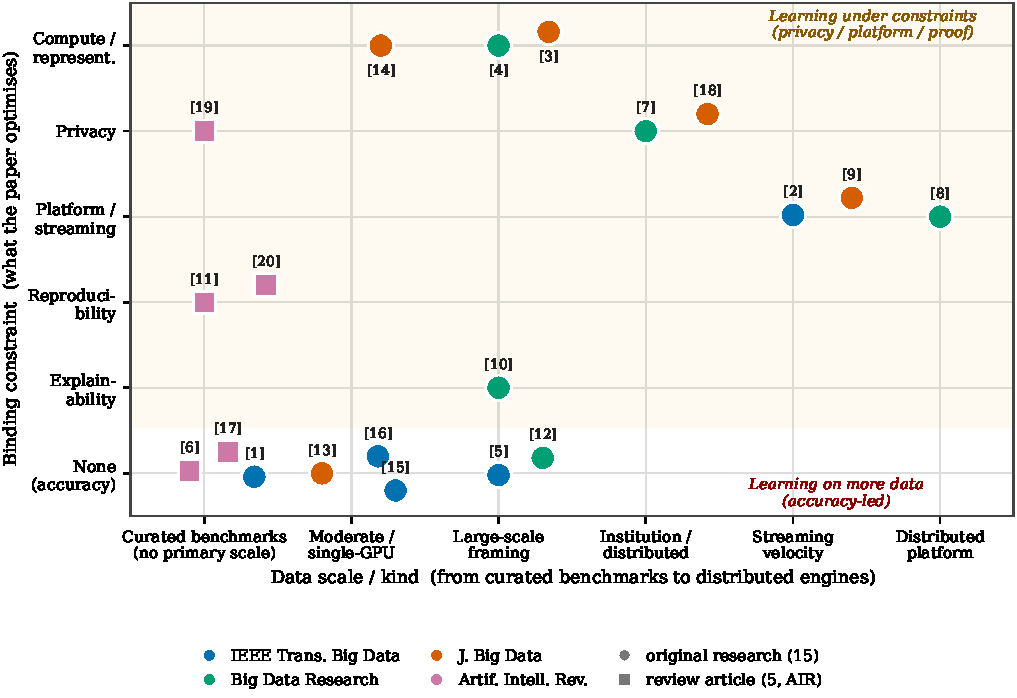
\includegraphics[width=\textwidth]{figures/fig1_corpus_landscape.pdf}
\caption{Corpus landscape. All 20 papers are placed on two chosen axes: data scale and kind (x) and binding constraint (y). Color marks the journal and marker shape separates research articles from review articles. Journal and article type are exact; the axis positions are interpretive design coordinates. The corpus splits into a lower band that learns on more data and an upper band that learns under constraints.}\label{fig1}
\end{figure*}

\begin{figure*}[t]
\centering
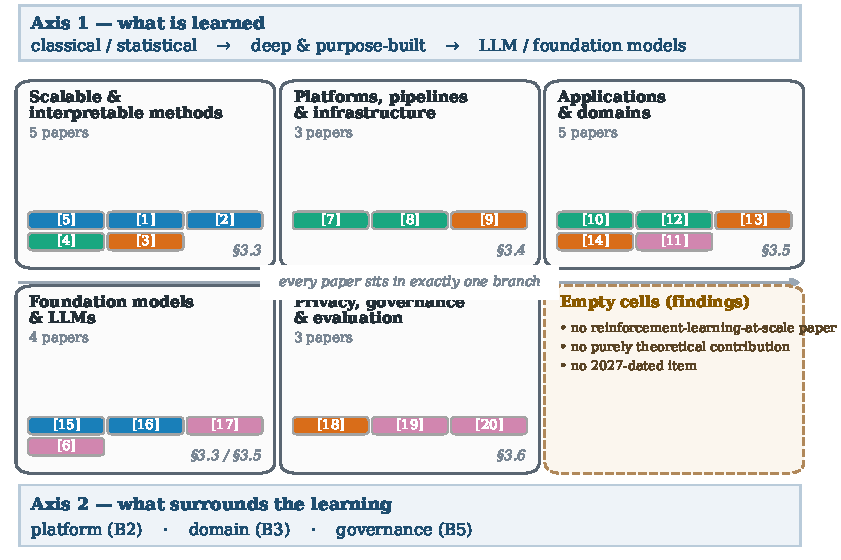
\includegraphics[width=\textwidth]{figures/fig2_taxonomy.pdf}
\caption{Two-axis taxonomy of the corpus. Axis~1 is what is learned; Axis~2 is what surrounds the learning. Five branches B1--B5 place each of the 20 papers exactly once, shown as citation numbers, for a total of 5+3+5+4+3. The branch assignment is this review's classification of this chosen corpus, and the empty cells (no reinforcement learning at scale, no purely theoretical contribution, no 2027 item) are findings rather than search gaps.}\label{fig2}
\end{figure*}

\begin{figure*}[t]
\centering
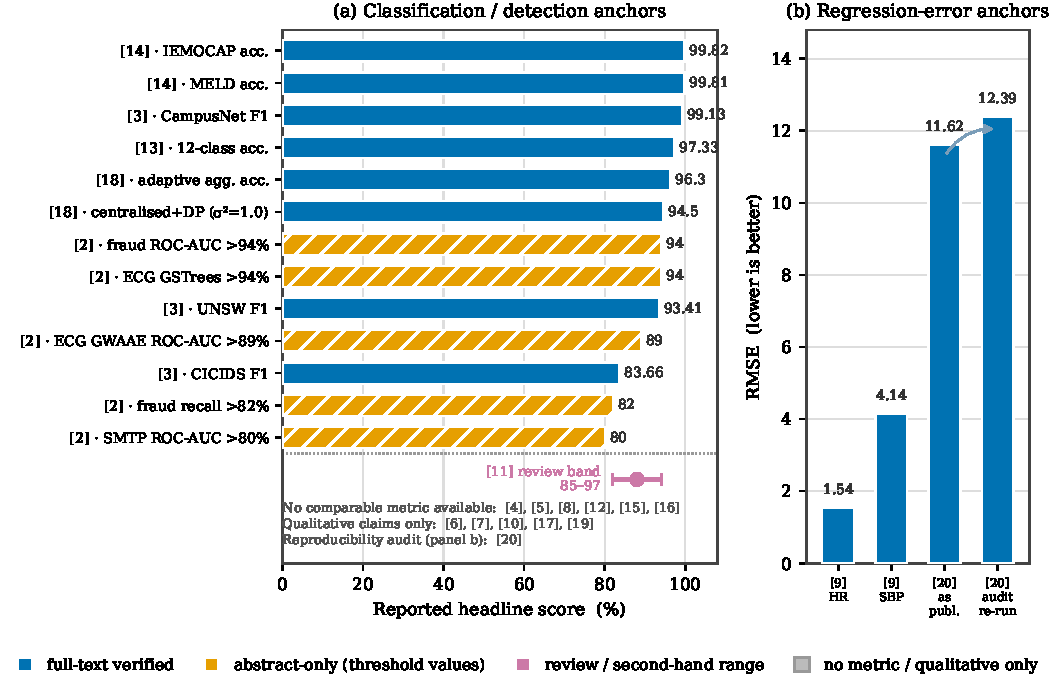
\includegraphics[width=\textwidth]{figures/fig3_evidence_anchors.pdf}
\caption{Reported-result anchors, not a like-for-like ranking. Panel (a) shows classification and detection values and panel (b) shows regression error with the corpus's only reported-to-reproduced pair. Values come from different datasets and metrics, so they are anchors rather than a leaderboard. Papers with no comparable metric are listed in a text band and are never plotted as zero. Hatching marks threshold values quoted from abstracts. The [14] accuracies (99.82\% and 99.81\%) are plotted as reported but are far above the emotion-recognition literature and are flagged as a reporting concern, not a capability result.}\label{fig3}
\end{figure*}

\begin{figure}[t]
\centering
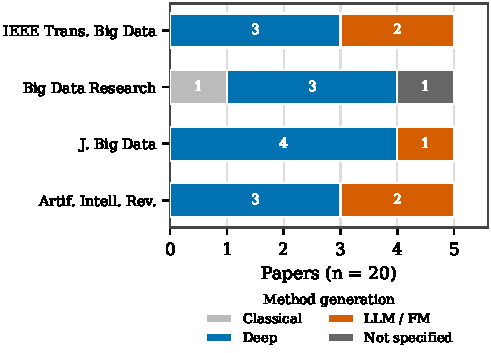
\includegraphics[width=0.9\columnwidth]{figures/fig4_method_shift.pdf}
\caption{Method-generation shift across the corpus by journal. Bars count the papers in each journal by method generation. The label is a chosen classification per paper, and ``not specified'' is kept visible rather than guessed, because one Big Data Research item reports no method detail in its published abstract. Each journal contributes five papers, so the bars are read as counts, not proportions.}\label{fig4}
\end{figure}

\begin{figure}[t]
\centering
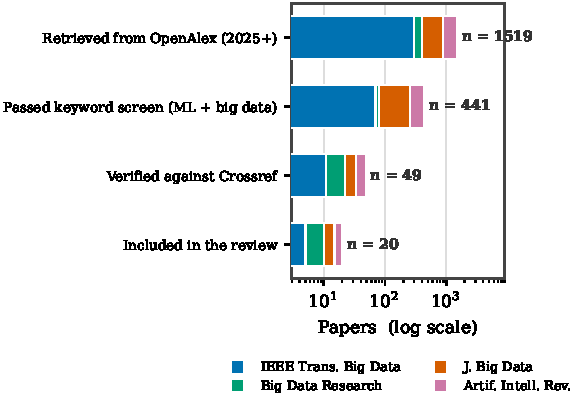
\includegraphics[width=0.9\columnwidth]{figures/fig5_selection_flow.pdf}
\caption{Selection flow for the corpus, in the style of a PRISMA funnel. Counts run from 1{,}519 items retrieved from the four journals (2025 or later) through a keyword filter at 441 and Crossref checks at 49 to 20 included papers, with a per-journal split of 5/5/5/5. The x-axis is log-scaled and labelled as such. The figure is descriptive and carries no performance claim.}\label{fig5}
\end{figure}

\section{Conclusion}\label{sec4}

This review examined 20 papers from four journals, five from each, and grouped them by theme. The corpus splits into five branches: scalable learning methods, platforms and pipelines, applications and domains, foundation models and language models, and privacy, governance, and evaluation. Across those branches, one claim held up. Big-data machine learning in this corpus has moved from learning on more data to learning under constraints, and those constraints are privacy, platform, and proof.

Three takeaways follow. The first is that constraint beats volume as the organizing problem. Four of the five methods papers improve a resource rather than a score: computation for the explainer and the classical estimator, latency for the streaming detectors, and representation efficiency for the graph embedding. The applications papers show the other side of the same coin, since several of them use ``big data'' for data variety or image volume while running on a single machine. The second takeaway is that privacy and scale collide, and the corpus does not settle the collision. Federated learning cuts data movement and protects locality, and it prices the cost: about 20\% savings in time and rounds in one framework, and an accuracy drop of two points under strong differential privacy. Centralized training assumes the opposite, and the streaming healthcare system leaves privacy out entirely. The third takeaway is that evaluation is the weakest joint. The corpus's only reproducibility audit shows that broad trends survive re-runs while exact numbers often do not, and the rest of the corpus reports single runs, abstract-level thresholds, or unattributed ranges.

The review has limits, and they bound the claim. The corpus is 20 papers from four journals in one two-year window, all in English, and the theme mix is chosen rather than sampled, so the branch proportions are not the field's proportions. For several of the 20 papers the published record is limited to an abstract, and a few report none at all, so those claims are stated at the level the available evidence supports rather than at full strength. Absence claims, such as the missing reinforcement-learning work, are scoped to this corpus and not to the field. A future review that covers the thinly reported items or widens the venue set could confirm or revise what this one reports. What this review can state is narrower and firmer: within a chosen 2025--2026 corpus of four journals, the field's binding limits are privacy, platform, and proof, and the corpus's own evidence, not the popular framing, shows it.

\backmatter

\bmhead{Acknowledgements}

Not applicable.

\section*{Declarations}

\begin{itemize}
\item Funding: Not applicable.
\item Conflict of interest: The authors declare no competing interests.
\item Ethics approval and consent to participate: Not applicable.
\item Consent for publication: Not applicable.
\item Data availability: The corpus is bibliographic. The 20 reviewed papers are identified by DOI in the reference list. Figure source data are available from the corresponding author on reasonable request.
\item Materials availability: Not applicable.
\item Code availability: The figures were produced with standard plotting software. No other code was developed for this review.
\item Author contribution: All authors contributed to the study. The corresponding author coordinated the review. Conception and design, literature screening, evidence extraction, thematic synthesis, and manuscript drafting were divided across the author team. All authors read and approved the final manuscript.
\end{itemize}

\bibliography{references}

\end{document}
